\documentclass{article}
\usepackage[utf8]{inputenc}
\usepackage{xcolor}
\usepackage{colortbl}
\usepackage{graphicx}
\usepackage{tikz}
\usepackage{lmodern}
\usepackage{amssymb,amsmath}
\usepackage{ifxetex,ifluatex}
\usepackage{fixltx2e} % provides \textsubscript
\usepackage{ngerman}
\usepackage{float}
\usepackage{caption}
\usepackage{subcaption}


\PassOptionsToPackage{hyphens}{url} % url is loaded by hyperref
\usepackage[unicode=true]{hyperref}

\usepackage{color}
\usepackage{fancyvrb}

\usepackage{mathtools}

\usepackage[a4paper, margin=3cm]{geometry}

\DeclarePairedDelimiter\floor{\lfloor}{\rfloor}
\newcommand*{\qed}{\hfill\ensuremath{\blacksquare}\\}%

% set default figure placement to htbp
\makeatletter

\title{FOP Projekt Wintersemester 2019/20}
\author{Yannik Sebastian Hayn, Julian Imhof,\\ Erik Prescher, Lennart Schmidt}
\makeatletter
\renewcommand*{\ps@plain}{%
  \let\@mkboth\@gobbletwo
  \let\@oddhead\@empty
  \def\@oddfoot{%
    \reset@font
    \hfil
    \thepage
    % \hfil % removed for aligning to the right
  }%
  \let\@evenhead\@empty
  \let\@evenfoot\@oddfoot
}
\usepackage{listings}
\lstset{language=Java,
  showspaces=false,
  showtabs=false,
  breaklines=true,
  showstringspaces=false,
  breakatwhitespace=true,
  basicstyle=\ttfamily
}
\makeatother
\pagestyle{plain}

\begin{document}
\maketitle
\section{Aufgabe 6.1.5 Theorie}
\subsection{Azyklischer Graph}
Da nur ein gerichteter Graph azyklisch sein kann, der hier gegebene Graph allerdings nicht gerichtet ist, kann er folglich auch nicht azyklisch sein.\\
 Im Folgenden gehen wir allerdings davon aus, dass auch ein nicht gerichteter Graph azyklisch sein k\"onne. Dabei nehmen wir an, dass ein Zyklus aus mindestens drei Nodes bestehen muss und der Zyklus \"uber $n - 1$ Kanten durchlaufen werden k\"onnen muss, ohne dabei zwei mal \"uber eine Kante zu gehen, wobei $n = Anzahl der Nodes$ ist.\\
Im Folgenden zeigen wir, dass der Graph zyklisch sein kann.\\

Betrachten wir uns zu Beginn einmal die einfachste Idee, um einen Zyklus zu erzeugen: Ein Kreisverkehr aus mehreren Stra{\ss}enkarten.
\begin{figure}[H]
	\centering
	\begin{subfigure}{.5\textwidth}
		\centering
		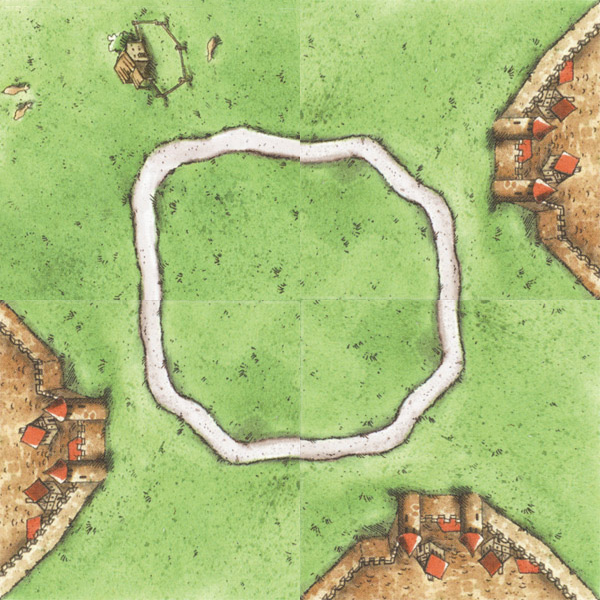
\includegraphics[width=0.9\textwidth]{Zyklischer_Graph.png}
		\caption{v.l.n.r. Pl\"attchen: V, J, J, J}
	\end{subfigure}%
	\begin{subfigure}{.5\textwidth}
		\centering
		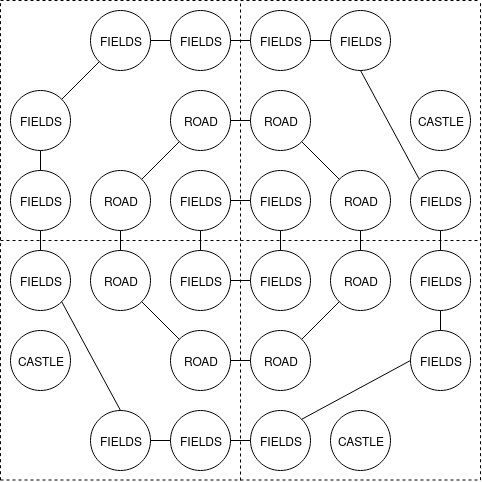
\includegraphics[width=0.9\textwidth]{Zyklischer_Graph1.png}
		\caption{zugeh\"origer Graph}
	\end{subfigure}
	\caption{Eine einfache M\"oglichkeit mit wenigen Pl\"attchen viele Zyklen zu erzeugen}
\end{figure}
Wie man direkt sehen kann, sind nur durch diese 4 Karten bereits 3 Zyklen entstanden.\qed

Wenn man diese Idee ein bisschen weiter f\"uhrt, kommt man relativ schnell zu dem Schluss, dass der Graph in den allermeisten F\"allen sp\"atestens bei Spielende zyklisch sein wird.


\end{document}
